\documentclass{beamer}
\usetheme{Boadilla}
\usepackage[utf8]{inputenc}
\usepackage{graphicx}
\graphicspath{ {./images/} }
\usepackage{hyperref}

\title{Version Control and Git}
\author{Augusto Fraga Giachero}
\date{\today}

\AtBeginSection[]{
  \begin{frame}
  \vfill
  \centering
  \begin{beamercolorbox}[sep=8pt,center,shadow=true,rounded=true]{title}
    \usebeamerfont{title}\insertsectionhead\par
  \end{beamercolorbox}
  \vfill
  \end{frame}
}

\begin{document}

% Title page frame
\begin{frame}
  \titlepage 
\end{frame}

% Outline frame
\begin{frame}{Outline}
  \tableofcontents
\end{frame}

\section{Version Control}

\subsection{In the Beginning}
\begin{frame}{In the Beginning}
  \begin{itemize}
    \item Collaborative software development required fine coordination between developers;
    \item Very hard to scale to large development teams;
    \item Versioning was a manual operation and error prone;
    \item No easy way to pinpoint modifications that introduced bugs;
    \item To avoid accidental data loss, backups had to be made often.
  \end{itemize}
\end{frame}

\subsection{Enter Version Control}
\begin{frame}{Enter Version Control}
  \begin{itemize}
    \item First widely used VCS: SCCS (developed in 1972 for OS/360, ported to UNIX afterwards, could only track single files);
    \item RCS, CVS and SVN followed (could track multiple files);
    \item Distributed VCS like BitKeeper, Git, Mercurial and Bazaar entered the scene a few years later.
  \end{itemize}
\end{frame}

\subsection{Version Control Concepts}
\begin{frame}{Version Control Concepts}
  \begin{itemize}
    \item Software to track modifications of a single file or a set of files (repository);
    \item Presents a history of states (commits) of a repository;
    \item Can store different history lines for the same repository (branches);
    \item Can synchronize modifications between branches (merging);
    \item Focused on tracking of plain-text files, but can offer binary file support, albeit with some limitations.
  \end{itemize}
\end{frame}

\subsection{Centralized Version Control}
\begin{frame}{Centralized Version Control}
  \begin{itemize}
    \item Requires a central server for almost all version control operations;
    \item Generally have the capability to 'lock files' to avoid concurrent modifications to the same file;
    \item Network access is required for collaborative development;
    \item No local branches.
  \end{itemize}
\end{frame}

\subsection{Distributed Version Control}
\begin{frame}{Distributed Version Control}
  \begin{itemize}
    \item There is no central server that coordinates commits, merges and other version control operations;
    \item Everything can be done locally, no network access required;
    \item All developers have a full copy of the repository history, resulting in a 'distributed backup' of the repository.
  \end{itemize}
\end{frame}

\section{Git}

\subsection{Git History}
\begin{frame}{Git History}
  \begin{itemize}
    \item In the beginning of 2005 the free license for BitKeeper (a proprietary VCS used by Linux kernel developers at time) was revoked;
    \item At the time, no open source VCS satisfied the requirements set up by Linus Torvalds of performance, distributed workflow, protections against accidental or malicious corruption;
    \item In April of 2005, Linus Torvalds started developing Git;
    \item In June of 2005, Git managed the Linux Kernel 2.6.12 release;
    \item Today Git is the predominant VCS used in software development.
  \end{itemize}
\end{frame}

\subsection{Git Design Goals}
\begin{frame}{Git Design Goals}
  \begin{itemize}
    \item High performance;
    \item Data integrity;
    \item Support distributed, non-linear workflows;
    \item Easy branching;
    \item Cryptographic protections against malicious data / history modification.
  \end{itemize}
\end{frame}

\subsection{Git Concepts}
\begin{frame}{Git Concepts}
  \begin{itemize}
    \item \textbf{Repository}: a directory containing the \texttt{.git} sub-directory and all files that can be tracked;
    \item \textbf{Commit}: a snapshot of a state of all \textbf{tracked} files in a repository. It also includes a message, author information, time and a pointer to the previous commit;
    \item \textbf{Branch}: a custom name to refer to a commit and its history;
    \item \textbf{Tag}: it is similar to a branch, but it is frozen in time (i.e. you can't add new commits to a tag);
    \item \textbf{Merge}: the action of combining the changes of one branch with another;
  \end{itemize}
\end{frame}

\subsection{Git Repository}
\begin{frame}{Git Repository}
  \begin{columns}
    \begin{column}{0.6\textwidth}
      \begin{itemize}
        \item The \texttt{.git} directory contains all files necessary to represent the history of the repository and other things (commits, branches, tags). \textbf{Not to be messed with};
        \item All files that can be tracked should be in the repository's directory or sub-directories;
        \item Files and directories that should not be tracked by Git (temporary files, build directories, etc) are specified in the \texttt{.gitignore} file.
      \end{itemize}
    \end{column}
    \begin{column}{0.4\textwidth}
      \begin{center}
        \begin{verbatim}
|-- .git
|   |-- ...
|-- .gitignore
|-- README.md
+-- src
    |-- main.c
    +-- Makefile
\end{verbatim}

      \end{center}
    \end{column}
  \end{columns}
\end{frame}

\subsection{Git Commits}
\begin{frame}{Git Commits}
  \begin{itemize}
    \item A commit refers to a state of all tracked files in a repository;
    \item It is unambiguously referred by its SHA-1 hash;
    \item It always has a reference to the previous commit (except when it is the first commit of a branch).
  \end{itemize}
  \begin{scriptsize}
    \begin{verbatim}
commit 51ad3af99a4e234aff70ab5046c099b46d8e7ee1
Author: Augusto Fraga Giachero <augusto.fraga@lnls.br>
Date:   Thu Sep 12 08:48:06 2024 -0300

    Remove CDC for adc_gains_fixed_point_pos register
    
    The adc_gains_fixed_point_pos is a constant, no need to cross clock
    domains. This fixes a problem when trying to read this register before
    initializing the fs_clk2x_i clock.
\end{verbatim}

  \end{scriptsize}
\end{frame}

\subsection{Git Branches}
\begin{frame}{Git Branches}
  \begin{columns}
    \begin{column}{0.6\textwidth}
      \begin{itemize}
        \item A branch is a pointer to a particular history of commits;
        \item It can be used to implement new features locally while other branches are been worked on by other developers;
        \item Another common usage is when maintaining different versions of a project (older stable releases get bugfixes while the new features are added to the 'unstable' branch).
      \end{itemize}
    \end{column}
    \begin{column}{0.4\textwidth}
      \begin{center}
        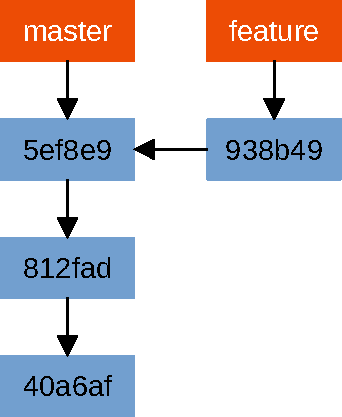
\includegraphics[scale=0.5]{git-branching}
      \end{center}
    \end{column}
  \end{columns}
\end{frame}

\subsection{Git Tags}
\begin{frame}{Git Tags}
  \begin{columns}
    \begin{column}{0.6\textwidth}
      \begin{itemize}
        \item Like a branch, a tag is a pointer to a particular history of commits;
        \item But tags are frozen, you can't add commits to a tag;
        \item Typically used to refer to project releases or pre-releases.
      \end{itemize}
    \end{column}
    \begin{column}{0.4\textwidth}
      \begin{center}
        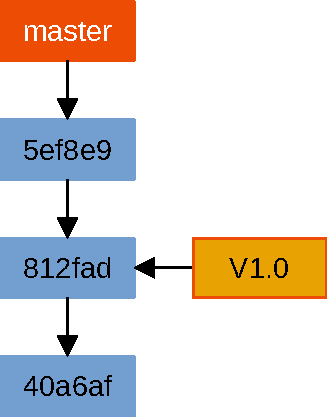
\includegraphics[scale=0.5]{git-tag}
      \end{center}
    \end{column}
  \end{columns}
\end{frame}

\subsection{Git Merges}
\begin{frame}{Git Merges}
  \begin{columns}
    \begin{column}{0.6\textwidth}
      \begin{itemize}
        \item There a three types of merge in git: standard merges (true merges), rebase merges and squash merges;
        \item All three perform the task of synchronizing the changes from one branch into another, but following different strategies.
      \end{itemize}
    \end{column}
    \begin{column}{0.4\textwidth}
      \begin{center}
        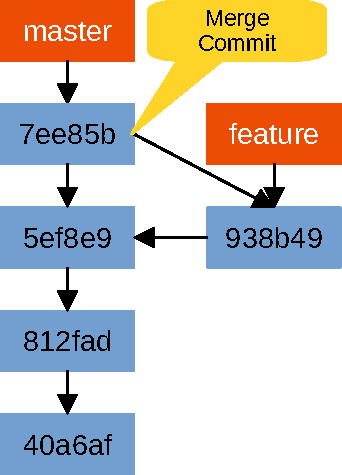
\includegraphics[scale=0.5]{git-merge}
      \end{center}
    \end{column}
  \end{columns}
\end{frame}

\subsection{Git Ignore}
\begin{frame}{Git Ignore}
  \begin{columns}
    \begin{column}{0.6\textwidth}
      \begin{itemize}
        \item It is common to have files or some file types that you don't want to track;
        \item To avoid accidentally commiting these, you can list the file names or file name patterns in the \texttt{.gitignore} file;
        \item The \texttt{.gitignore} file pattern list will be applied recursively to all child directories.
      \end{itemize}
    \end{column}
    \begin{column}{0.4\textwidth}
      \begin{flushright}
        \begin{verbatim}
# Emacs temporary files
*~
\#*\#
.\#*
\end{verbatim}

      \end{flushright}
    \end{column}
  \end{columns}
\end{frame}

\begin{frame}{Contact}
  email: \href{mailto:augusto.fraga@lnls.br}{augusto.fraga@lnls.br} \\
  Github page: \url{github.com/augustofg}
  \begin{center}
    Thanks!
  \end{center}
\end{frame}

\end{document}
